% Options for packages loaded elsewhere
\PassOptionsToPackage{unicode}{hyperref}
\PassOptionsToPackage{hyphens}{url}
\PassOptionsToPackage{dvipsnames,svgnames,x11names}{xcolor}
%
\documentclass[
]{article}

\usepackage{amsmath,amssymb}
\usepackage{iftex}
\ifPDFTeX
  \usepackage[T1]{fontenc}
  \usepackage[utf8]{inputenc}
  \usepackage{textcomp} % provide euro and other symbols
\else % if luatex or xetex
  \usepackage{unicode-math}
  \defaultfontfeatures{Scale=MatchLowercase}
  \defaultfontfeatures[\rmfamily]{Ligatures=TeX,Scale=1}
\fi
\usepackage{lmodern}
\ifPDFTeX\else  
    % xetex/luatex font selection
\fi
% Use upquote if available, for straight quotes in verbatim environments
\IfFileExists{upquote.sty}{\usepackage{upquote}}{}
\IfFileExists{microtype.sty}{% use microtype if available
  \usepackage[]{microtype}
  \UseMicrotypeSet[protrusion]{basicmath} % disable protrusion for tt fonts
}{}
\makeatletter
\@ifundefined{KOMAClassName}{% if non-KOMA class
  \IfFileExists{parskip.sty}{%
    \usepackage{parskip}
  }{% else
    \setlength{\parindent}{0pt}
    \setlength{\parskip}{6pt plus 2pt minus 1pt}}
}{% if KOMA class
  \KOMAoptions{parskip=half}}
\makeatother
\usepackage{xcolor}
\setlength{\emergencystretch}{3em} % prevent overfull lines
\setcounter{secnumdepth}{-\maxdimen} % remove section numbering
% Make \paragraph and \subparagraph free-standing
\makeatletter
\ifx\paragraph\undefined\else
  \let\oldparagraph\paragraph
  \renewcommand{\paragraph}{
    \@ifstar
      \xxxParagraphStar
      \xxxParagraphNoStar
  }
  \newcommand{\xxxParagraphStar}[1]{\oldparagraph*{#1}\mbox{}}
  \newcommand{\xxxParagraphNoStar}[1]{\oldparagraph{#1}\mbox{}}
\fi
\ifx\subparagraph\undefined\else
  \let\oldsubparagraph\subparagraph
  \renewcommand{\subparagraph}{
    \@ifstar
      \xxxSubParagraphStar
      \xxxSubParagraphNoStar
  }
  \newcommand{\xxxSubParagraphStar}[1]{\oldsubparagraph*{#1}\mbox{}}
  \newcommand{\xxxSubParagraphNoStar}[1]{\oldsubparagraph{#1}\mbox{}}
\fi
\makeatother


\providecommand{\tightlist}{%
  \setlength{\itemsep}{0pt}\setlength{\parskip}{0pt}}\usepackage{longtable,booktabs,array}
\usepackage{calc} % for calculating minipage widths
% Correct order of tables after \paragraph or \subparagraph
\usepackage{etoolbox}
\makeatletter
\patchcmd\longtable{\par}{\if@noskipsec\mbox{}\fi\par}{}{}
\makeatother
% Allow footnotes in longtable head/foot
\IfFileExists{footnotehyper.sty}{\usepackage{footnotehyper}}{\usepackage{footnote}}
\makesavenoteenv{longtable}
\usepackage{graphicx}
\makeatletter
\def\maxwidth{\ifdim\Gin@nat@width>\linewidth\linewidth\else\Gin@nat@width\fi}
\def\maxheight{\ifdim\Gin@nat@height>\textheight\textheight\else\Gin@nat@height\fi}
\makeatother
% Scale images if necessary, so that they will not overflow the page
% margins by default, and it is still possible to overwrite the defaults
% using explicit options in \includegraphics[width, height, ...]{}
\setkeys{Gin}{width=\maxwidth,height=\maxheight,keepaspectratio}
% Set default figure placement to htbp
\makeatletter
\def\fps@figure{htbp}
\makeatother

\usepackage{float}
\usepackage{tabularray}
\usepackage[normalem]{ulem}
\usepackage{graphicx}
\UseTblrLibrary{booktabs}
\UseTblrLibrary{rotating}
\UseTblrLibrary{siunitx}
\NewTableCommand{\tinytableDefineColor}[3]{\definecolor{#1}{#2}{#3}}
\newcommand{\tinytableTabularrayUnderline}[1]{\underline{#1}}
\newcommand{\tinytableTabularrayStrikeout}[1]{\sout{#1}}
\makeatletter
\@ifpackageloaded{caption}{}{\usepackage{caption}}
\AtBeginDocument{%
\ifdefined\contentsname
  \renewcommand*\contentsname{Table of contents}
\else
  \newcommand\contentsname{Table of contents}
\fi
\ifdefined\listfigurename
  \renewcommand*\listfigurename{List of Figures}
\else
  \newcommand\listfigurename{List of Figures}
\fi
\ifdefined\listtablename
  \renewcommand*\listtablename{List of Tables}
\else
  \newcommand\listtablename{List of Tables}
\fi
\ifdefined\figurename
  \renewcommand*\figurename{Figure}
\else
  \newcommand\figurename{Figure}
\fi
\ifdefined\tablename
  \renewcommand*\tablename{Table}
\else
  \newcommand\tablename{Table}
\fi
}
\@ifpackageloaded{float}{}{\usepackage{float}}
\floatstyle{ruled}
\@ifundefined{c@chapter}{\newfloat{codelisting}{h}{lop}}{\newfloat{codelisting}{h}{lop}[chapter]}
\floatname{codelisting}{Listing}
\newcommand*\listoflistings{\listof{codelisting}{List of Listings}}
\makeatother
\makeatletter
\makeatother
\makeatletter
\@ifpackageloaded{caption}{}{\usepackage{caption}}
\@ifpackageloaded{subcaption}{}{\usepackage{subcaption}}
\makeatother

\ifLuaTeX
  \usepackage{selnolig}  % disable illegal ligatures
\fi
\usepackage{bookmark}

\IfFileExists{xurl.sty}{\usepackage{xurl}}{} % add URL line breaks if available
\urlstyle{same} % disable monospaced font for URLs
\hypersetup{
  pdftitle={HW5},
  pdfauthor={Miracle Ephraim},
  colorlinks=true,
  linkcolor={blue},
  filecolor={Maroon},
  citecolor={Blue},
  urlcolor={Blue},
  pdfcreator={LaTeX via pandoc}}


\title{HW5}
\author{Miracle Ephraim}
\date{}

\begin{document}
\maketitle


\textbf{Github Repository:}
\url{https://github.com/miracleephraim/hw5.git}

\subsection{Question 1}\label{question-1}

Plot the share of the adult population with direct purchase health
insurance over time.

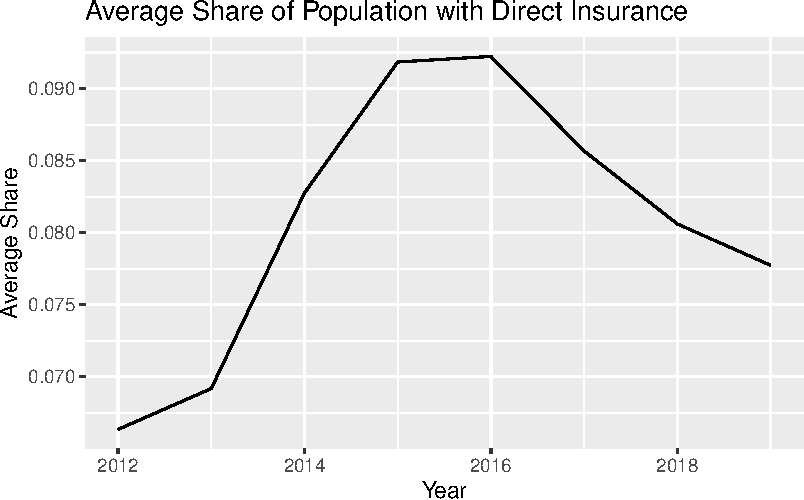
\includegraphics{ephraim-m-hwk5-1_files/figure-pdf/unnamed-chunk-1-1.pdf}

\subsection{Question 2}\label{question-2}

Discuss the reduction in direct purchase health insurance in later
years. Can you list a couple of policies that might have affected the
success of the direct purchase insurance market?

Following 2016, there is a continous decrease in the share of the
populaiton directly purchasing health insurance, likely due to the ACA.
After 2016, the elimination of the penalty on those without health
insurance, which likely reduced the incentive to purchase health
insurance. In these latter years, the Trump administration ended federal
cost-sharing reduction payments, which also de-incentvized direct
purchase as premiums increases for those without subsidies
\href{https://www.kff.org/private-insurance/issue-brief/as-aca-marketplace-enrollment-reaches-record-high-fewer-are-buying-individual-market-coverage-elsewhere/\#:~:text=During\%20this\%20period\%20of\%20decreasing,Figure\%201}{(1,}
\href{https://usafacts.org/articles/affordable-care-act-and-data-who-insured-and-who-isnt/\#:~:text=Individual\%20mandate,Employer\%20mandate}{2).}

\subsection{Question 3}\label{question-3}

Plot the share of the adult population with Medicaid over time.

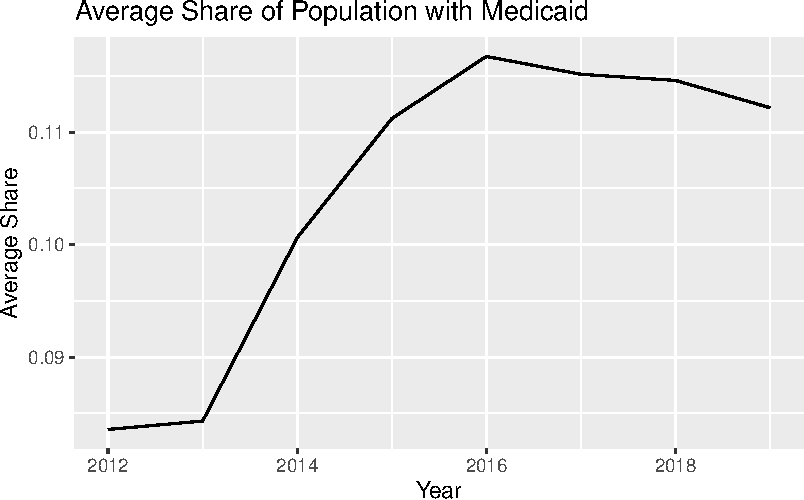
\includegraphics{ephraim-m-hwk5-1_files/figure-pdf/unnamed-chunk-2-1.pdf}

\subsection{Question 4}\label{question-4}

Plot the share of uninsured over time, separately by states that
expanded Medicaid in 2014 versus those that did not. Drop all states
that expanded after 2014.

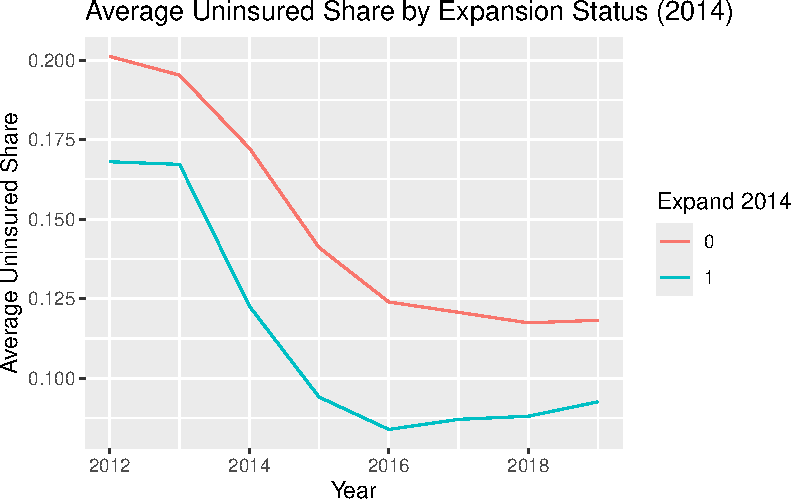
\includegraphics{ephraim-m-hwk5-1_files/figure-pdf/unnamed-chunk-3-1.pdf}

\subsection{Question 5}\label{question-5}

Calculate the average percent of uninsured individuals in 2012 and 2015,
separately for expansion and non-expansion states. Present your results
in a basic 2x2 DD table.

\begin{longtable}[]{@{}lll@{}}
\toprule\noalign{}
& Pre-Period (2012) & Post-Period (2015) \\
\midrule\noalign{}
\endhead
\bottomrule\noalign{}
\endlastfoot
Expansion States & NA & 9.81\% \\
Non-Expansion States & 18.7\% & 15.3\% \\
\end{longtable}

\subsection{Question 6}\label{question-6}

Estimate the effect of Medicaid expansion on the uninsurance rate using
a standard DD regression estimator, again focusing only on states that
expanded in 2014 versus those that never expanded.

\begin{table}
\centering
\begin{talltblr}[         %% tabularray outer open
entry=none,label=none,
note{}={+ p \num{< 0.1}, * p \num{< 0.05}, ** p \num{< 0.01}, *** p \num{< 0.001}},
]                     %% tabularray outer close
{                     %% tabularray inner open
colspec={Q[]Q[]},
column{2}={}{halign=c,},
column{1}={}{halign=l,},
}                     %% tabularray inner close
\toprule
& DD (2014) \\ \midrule %% TinyTableHeader
postTRUE & \num{-0.054}*** \\
& (\num{0.003}) \\
expand\_everTRUE & \num{-0.046}** \\
& (\num{0.016}) \\
postTRUE × expand\_everTRUE & \num{-0.019}** \\
& (\num{0.007}) \\
\bottomrule
\end{talltblr}
\end{table}

\subsection{Question 7}\label{question-7}

Include state and year fixed effects in your estimates. Try using the
lfe or fixest package to estimate this instead of directly including the
fixed effects.

\begin{table}
\centering
\begin{talltblr}[         %% tabularray outer open
entry=none,label=none,
note{}={+ p \num{< 0.1}, * p \num{< 0.05}, ** p \num{< 0.01}, *** p \num{< 0.001}},
]                     %% tabularray outer close
{                     %% tabularray inner open
colspec={Q[]Q[]Q[]},
column{2,3}={}{halign=c,},
column{1}={}{halign=l,},
}                     %% tabularray inner close
\toprule
& DD & TWFE \\ \midrule %% TinyTableHeader
postTRUE & \num{-0.054}*** &  \\
& (\num{0.003}) &  \\
expand\_everTRUE & \num{-0.046}** &  \\
& (\num{0.016}) &  \\
postTRUE × expand\_everTRUE & \num{-0.019}** &  \\
& (\num{0.007}) &  \\
treat &  & \num{-0.019}* \\
&  & (\num{0.007}) \\
\bottomrule
\end{talltblr}
\end{table}

\subsection{Question 8}\label{question-8}

Repeat the analysis in question 7 but include all states (even those
that expanded after 2014). Are your results different? If so, why?

\begin{table}
\centering
\begin{talltblr}[         %% tabularray outer open
entry=none,label=none,
note{}={+ p \num{< 0.1}, * p \num{< 0.05}, ** p \num{< 0.01}, *** p \num{< 0.001}},
]                     %% tabularray outer close
{                     %% tabularray inner open
colspec={Q[]Q[]Q[]Q[]Q[]},
column{2,3,4,5}={}{halign=c,},
column{1}={}{halign=l,},
}                     %% tabularray inner close
\toprule
& DD (2014) & TWFE (2014) & DD (all) & TWFE (all) \\ \midrule %% TinyTableHeader
postTRUE & \num{-0.054}*** &  & \num{-0.054}*** &  \\
& (\num{0.003}) &  & (\num{0.003}) &  \\
expand\_everTRUE & \num{-0.046}** &  & \num{-0.040}** &  \\
& (\num{0.016}) &  & (\num{0.015}) &  \\
postTRUE × expand\_everTRUE & \num{-0.019}** &  & \num{-0.017}** &  \\
& (\num{0.007}) &  & (\num{0.006}) &  \\
treat &  & \num{-0.019}* &  & \num{-0.017}** \\
&  & (\num{0.007}) &  & (\num{0.006}) \\
\bottomrule
\end{talltblr}
\end{table}

Results are different, but not by a significant magnitude. This is
likely due to the added states not significantly altering the overall
trends and the lack of the correct event study time fails to capture the
full effects of expansion implementation.

\subsection{Question 9}\label{question-9}

Provide an ``event study'' graph showing the effects of Medicaid
expansion in each year. Use the specification that includes state and
year fixed effects, limited to states that expanded in 2014 or never
expanded.

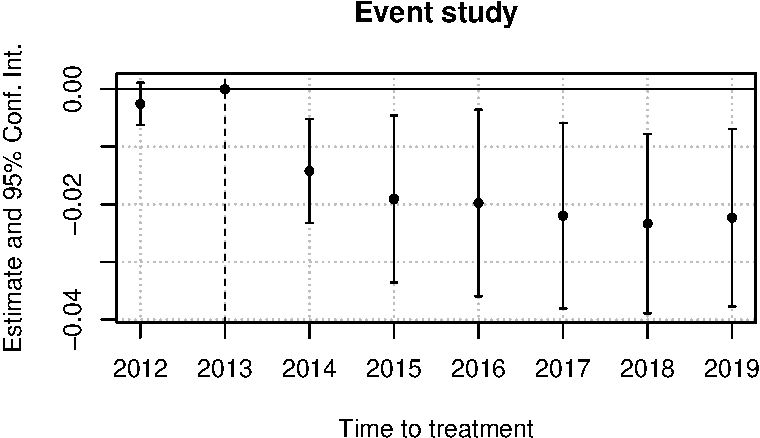
\includegraphics{ephraim-m-hwk5-1_files/figure-pdf/unnamed-chunk-7-1.pdf}

\subsection{Question 10}\label{question-10}

Repeat part 9 but again include states that expanded after 2014. Note:
this is tricky\ldots you need to put all states onto ``event time'' to
create this graph.

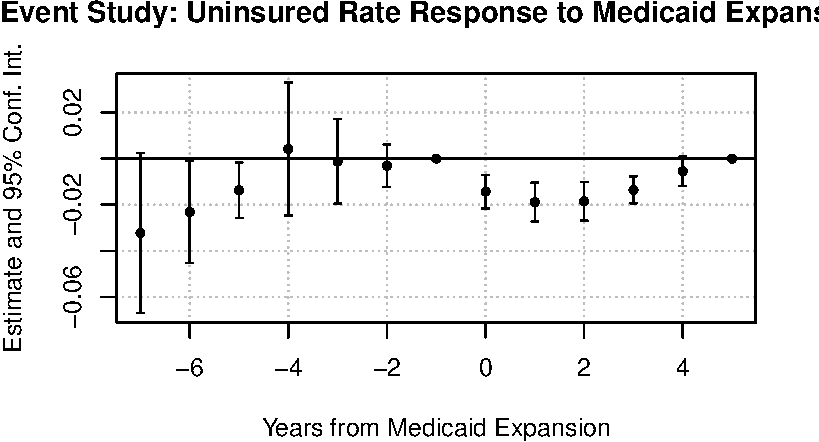
\includegraphics{ephraim-m-hwk5-1_files/figure-pdf/unnamed-chunk-8-1.pdf}




\end{document}
